%!TEX root = main.tex

\section{Background}
\label{sec:background}

In this section, we motivate the benefits of continuous training of DNN models that are deployed in the field for video inferences (\S\ref{subsec:continuous}), and then explain the setup for doing such continuous training on edge devices (\S\ref{subsec:edge}).

\subsection{Continuous Training}
\label{subsec:continuous}

% use cases - connected smart cars, indexing on iphone, even stationary traffic cameras
Advances in DNN efficiency, for example, using model compression \cite{compression1, compression2}, have enabled the deployment of DNN models on edge devices. Efficient edge models drive many video analytics applications in smart cars, mobile devices, and enterprise campuses. Video analytics in smart cars already provides safety assist features (e.g., lane drift alerts) and more features are expected \cite{smart-cars}. Camera streams in enterprise buildings are analyzed for traditional security applications as well as for ubiquitous sensing applications, e.g., face recognition to authenticate building access \cite{smart-buildings}. Mobile devices use DNN object classifiers to generate ``tags'' for the pictures and videos clicked by users, thus enabling search by keywords (e.g., find pictures with a party hat) \cite{iphone-indexing}. 
\junchen{this para could be a good fit to a new subsection of ``DNN deployed at the edge''?}
\junchen{i like the idea of starting with data drift, though maybe we should motivate why data drift is so damaging in the first place? }

\noindent{\bf Data drift.} %While model compression has considerably increased the inference efficiency of DNN models, it also results in their having lower ``capacity'' to learn from their training data. 
While compressed models are initially trained on representative data samples, when they are out in the field, they encounter the well-documented phenomenon of {\em data drift} \cite{drift1, drift2}. Data drift refers to the phenomenon of the live video data becoming significantly different than the data used to train the edge model. For example, the camera in a car observes vastly varying scenes (lighting, backgrounds, etc.) as it moves around different neighborhoods, thus making it difficult to accurately classify the objects of interest (like cars and bicycles). Further, newer object classes start appearing (e.g., segway scooters) which may not have been included in the initial training data. It is generally difficult to provide an exhaustive training dataset encompassing enough samples of all possible object classes. \ga{Model capacity drops due to compression?} \junchen{to Ganesh's comment on compression vs. capacity: totally agree this is what any (knowledgeable) reviewer may wonder as well. i believe there {\em is} a fundamental tradeoff between capacity (how much to compress) and generalizability (robustness to data drift).
maybe just cite the ECCV paper Romil found and ask Nikolas for more.} \ys{+1 on this point. The large the model is, the higher capacity it has. However, a large model not only requires a huge amount of data and time for training, but also leads to a higher runtime cost (memory, latency etc.) during inference. Hence, an alternative of having a large well-trained model is to maintain a localized cheaper model, and retrain it on demand. }

The preferred approach, instead, is for edge models to {\em continuously learn} as they incrementally observe new data samples with time. Incremental learning has indeed gained significant attention in the machine learning community \cite{incremental1, incremental2, incremental3}. Incremental learning techniques retain snapshots of history for the retraining (not the entire historical dataset) and avoid {\em catastrophic forgetting} of the learnings on historical data \cite{catastrophic} even as they learn from new data samples. In our work, we adopt the \gaa{XXX}.

% data drift; class incremental; waymo graphs; app-level impact
\noindent{\bf Accuracy benefit to retraining.} We use the Cityscapes and Waymo datasets \cite{sun2019scalability, cityscapes} to demonstrate the value of continuous learning. Cityscapes dataset is obtained from dashboard cameras in cars driving around many cities in Europe \cite{cityscapes}. The Waymo dataset is obtained from dashboard cameras in cars driving around multiple cities in the US \cite{sun2019scalability}. In both datasets, cameras obtain new data samples and encounter new object classes with time, thus requiring continuous learning for the DNNs. (More details of the datasets can be found in \S\ref{subsec:eval-setup}). 


% sample incremental; jena and tubingen of cityscapes
Figure \ref{fig:cityscapes-motivation} shows the benefits of {\em sample-incremental} training, i.e., improving the model with newer data samples over time, on the Cityscapes dataset. %We use two videos for this experiments from cars driving in two cities, Jena and Tubingen. 
We compare the accuracies of the constantly updated ResNet18 convolutional classifier against the version of ResNet18 that was trained only once \romilc{on a few samples of the data domain (say, by collecting a representative sample before the edge model was deployed)} but never updated. We evaluate the accuracy of the dominant classes -- 'person', 'car, 'truck', 'bus', 'bicycle', 'motorcycle' -- in % and the class distribution does not change with time in 
Figure \ref{fig:cityscapes-motivation}. 

As we can see in Figure \ref{fig:jena-motivation}, while the accuracies of the two models are similar at the beginning, they diverge over time to a difference of as much as $20\%$ in accuracy. Continuous updates of the model (learning from new data samples) results in its accuracy remaining steady over time and higher compared to the model that is not updated continuously. We observe a similar trend in Figure \ref{fig:tubingen-motivation} where the difference in accuracy due to not updating the model is observed immediately. Overall, Figure \ref{fig:cityscapes-motivation} highlights the value of improving the models with new {\em samples}, even when the classes of interest do not change.
\junchen{hmm.. i do see the point that having more samples helps, but in any event, people will use a model (even a cheap one) trained offline with some {\em large} standard dataset (imagenet, coco, etc). i tend to believe the gain is due to fine-tuning the ResNet model to in-situ data from the Cityscape ``scene'' and more such data the better?}

\begin{figure}[t]
  \centering
%   \begin{subfigure}[b]{0.5\linewidth}
%     \centering
%     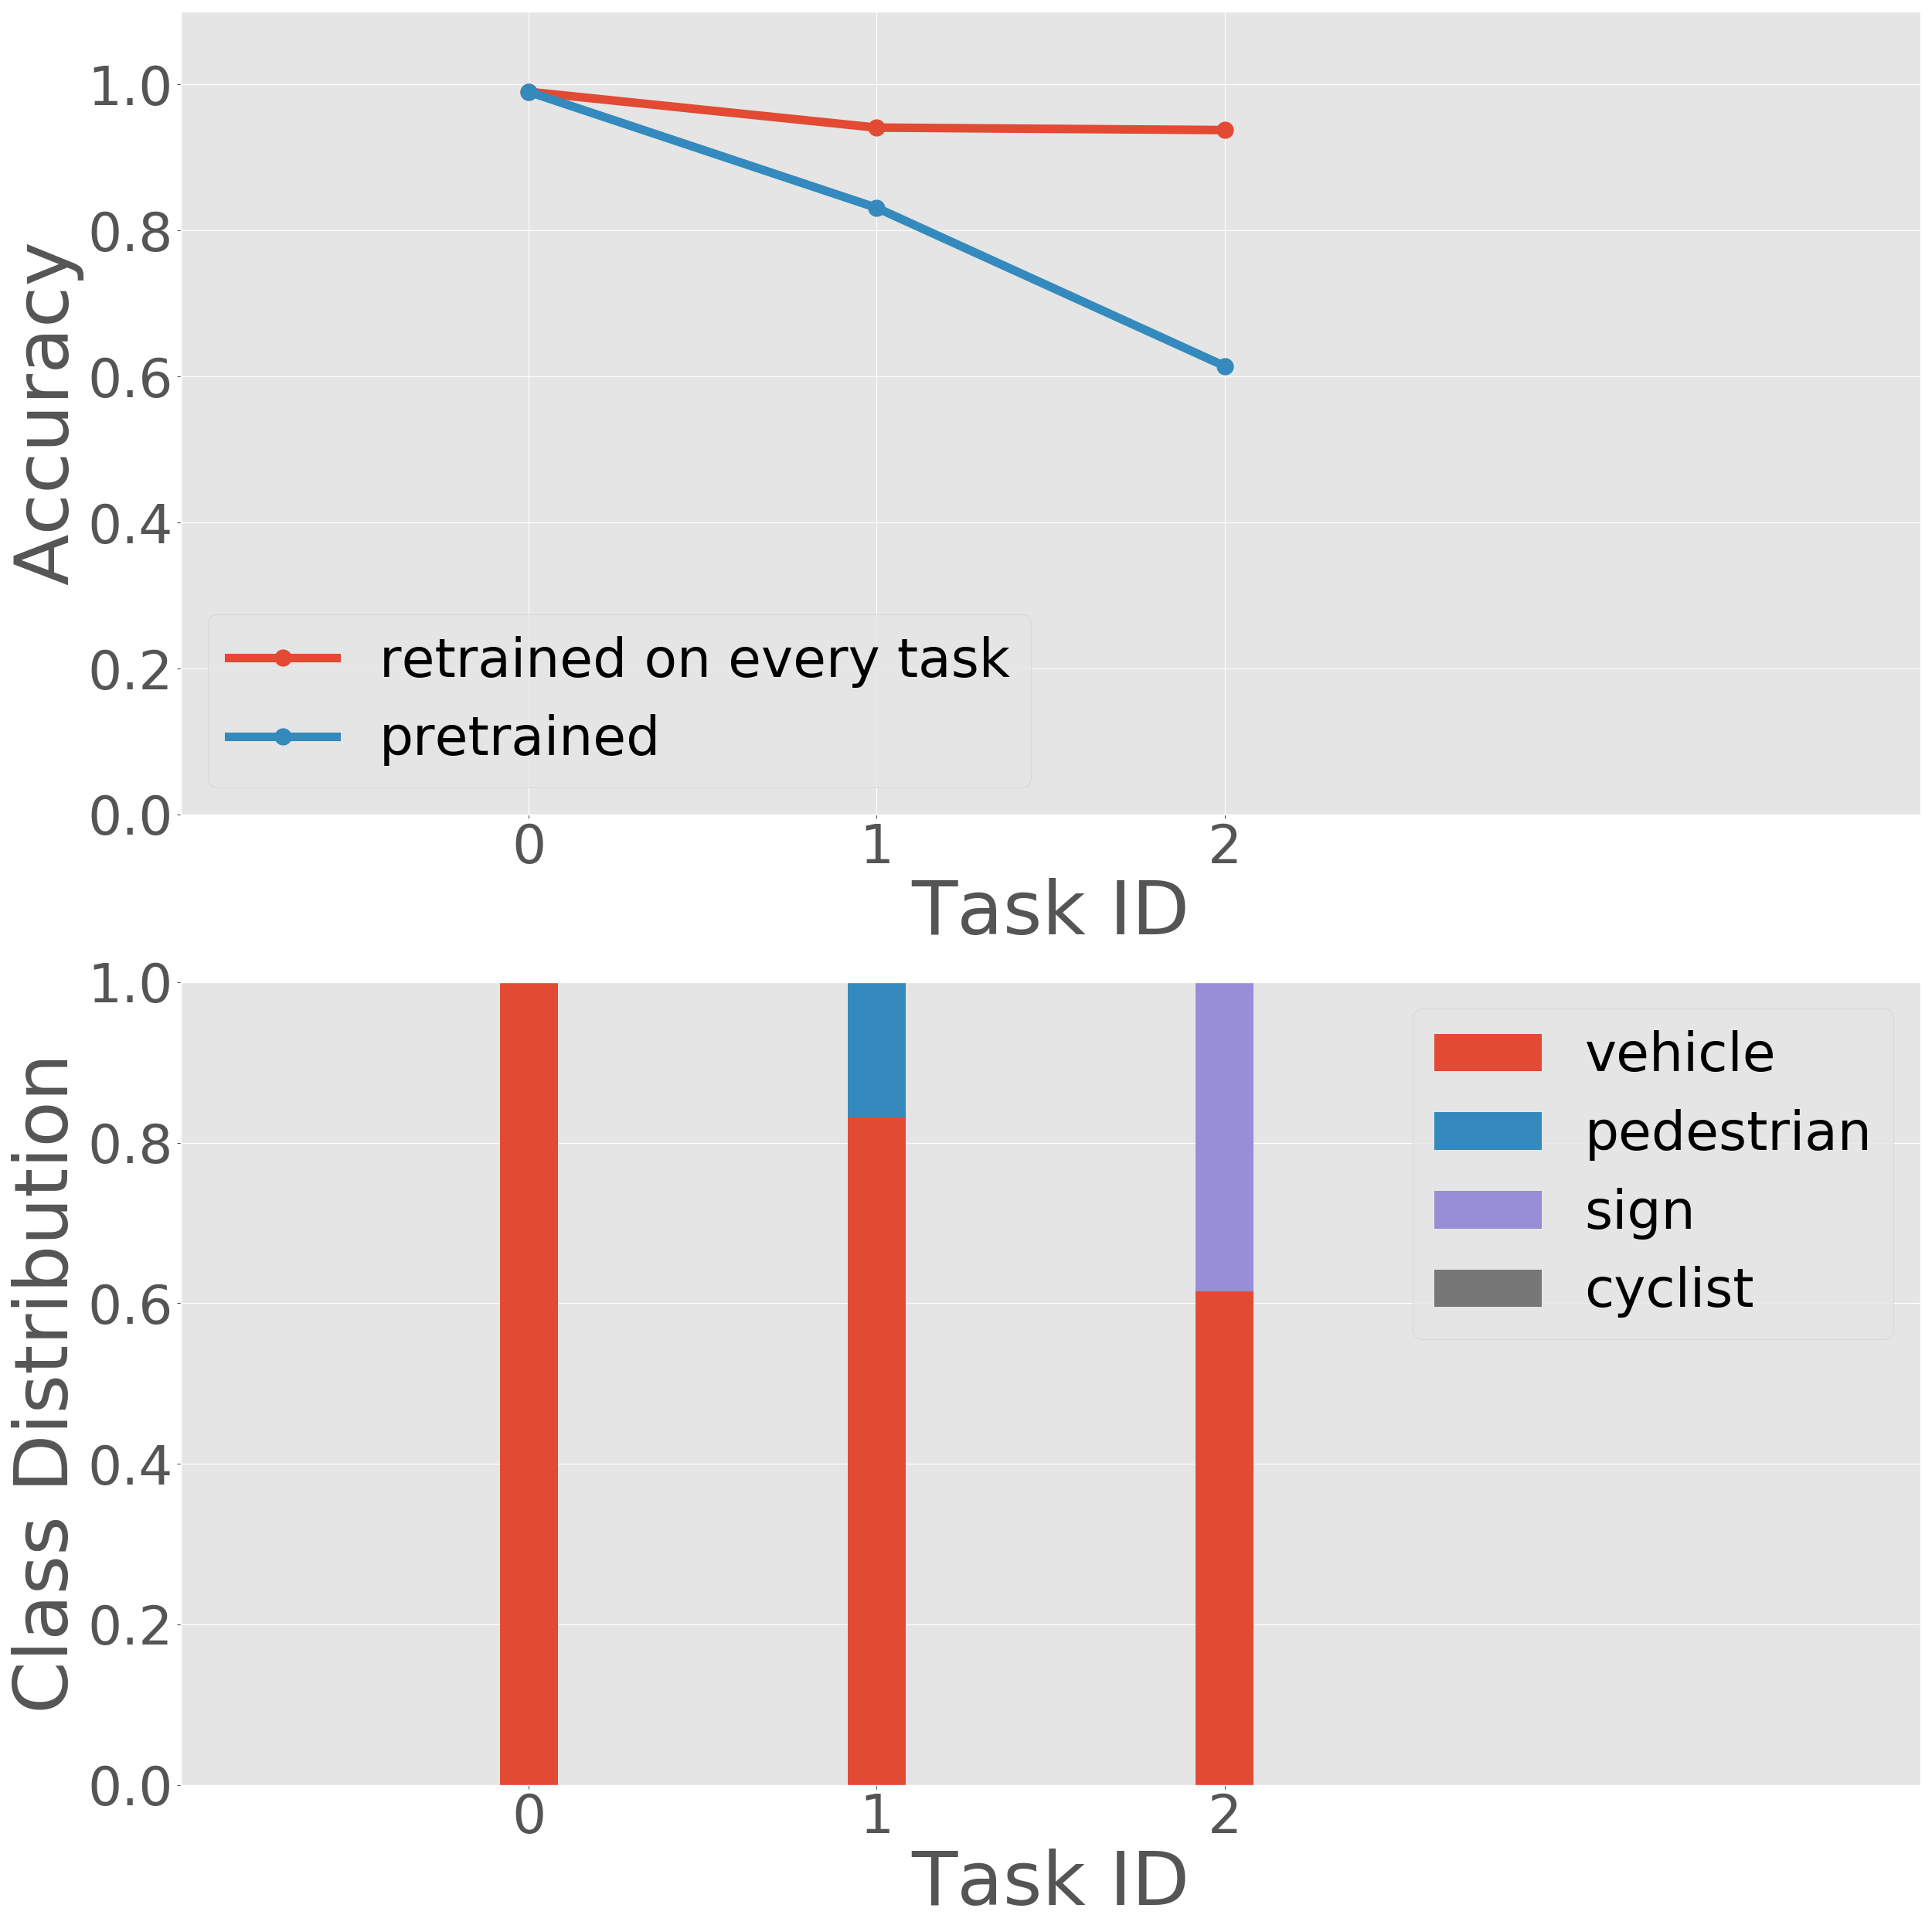
\includegraphics[width=\linewidth]{figures/motivation/Class_Incrementality/new_x_phx_234.png}
%     \caption{New classes show up over time}
%     \label{fig:new-classes-motivation}
%   \end{subfigure}  
\begin{subfigure}[t]{0.5\linewidth}
    \centering
    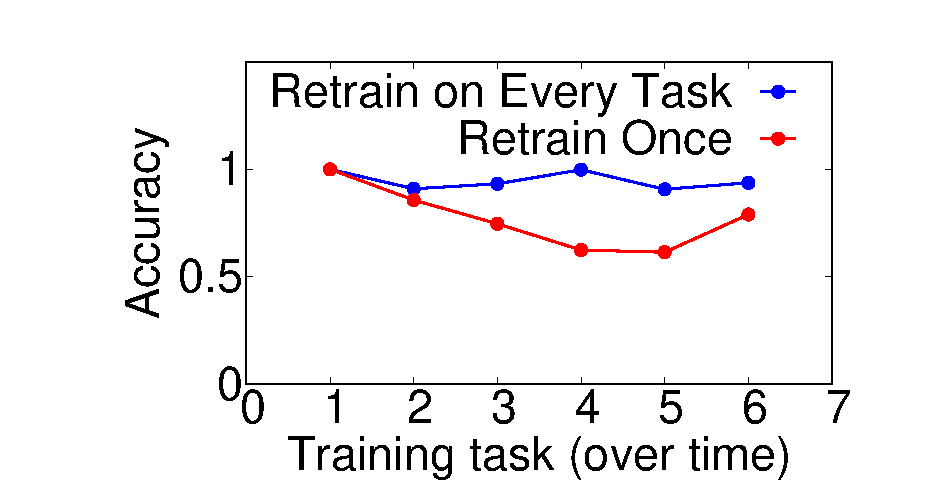
\includegraphics[width=\linewidth]{figures/motivation/Class_Incrementality/new_class_acc.eps}
  \end{subfigure}
%   \hfill
  ~~
  \begin{subfigure}[t]{0.5\linewidth}
    \centering
    % 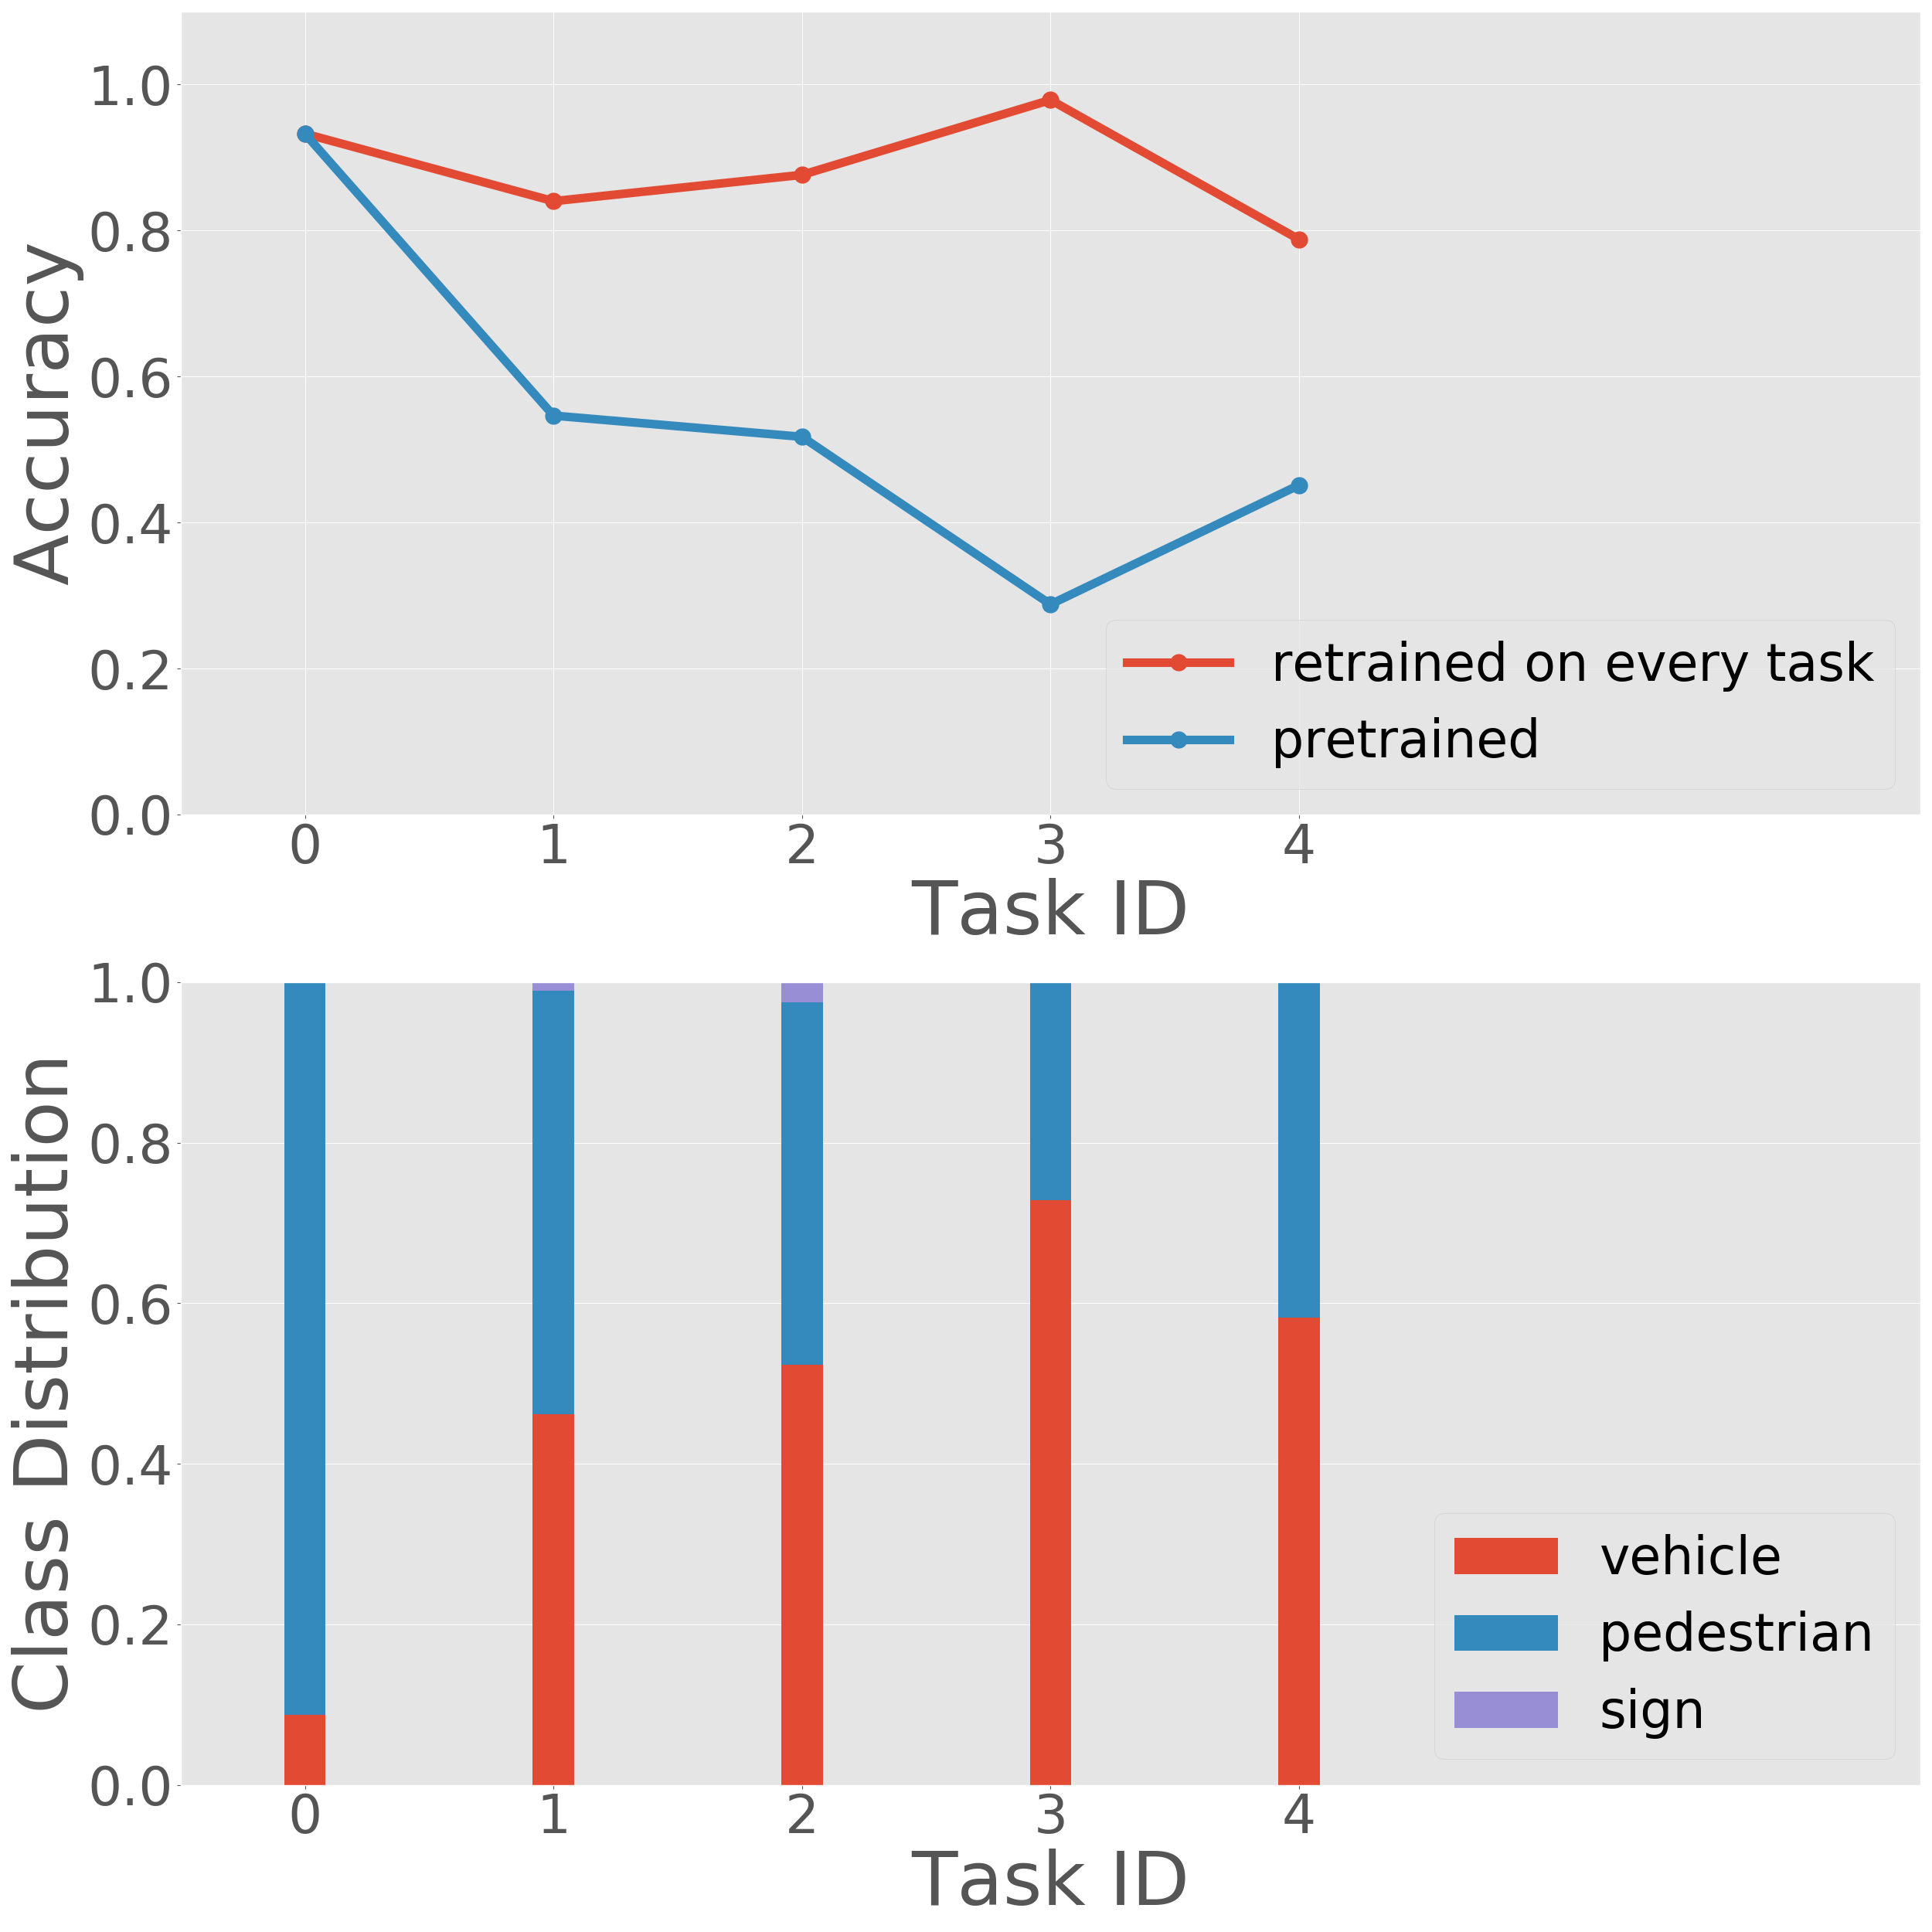
\includegraphics[width=\linewidth]{figures/motivation/Class_Incrementality/class_distribution_change_sf_27.png}
    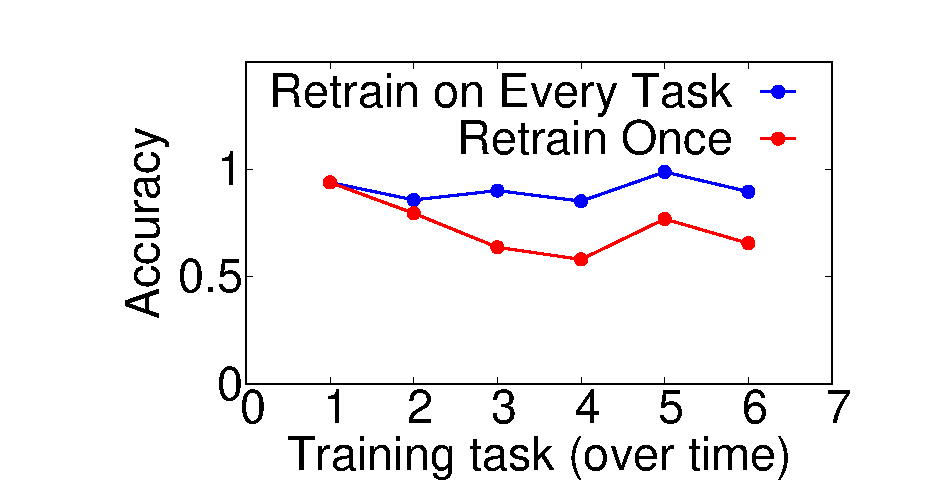
\includegraphics[width=\linewidth]{figures/motivation/Class_Incrementality/class_dist_change_acc.eps}
    % \caption{Class distribution varies over time}
    \label{fig:class-distrib-motivation-acc}
  \end{subfigure}
%   \medskip
% %   ~~
  \begin{subfigure}[t]{0.5\linewidth}
    \centering
    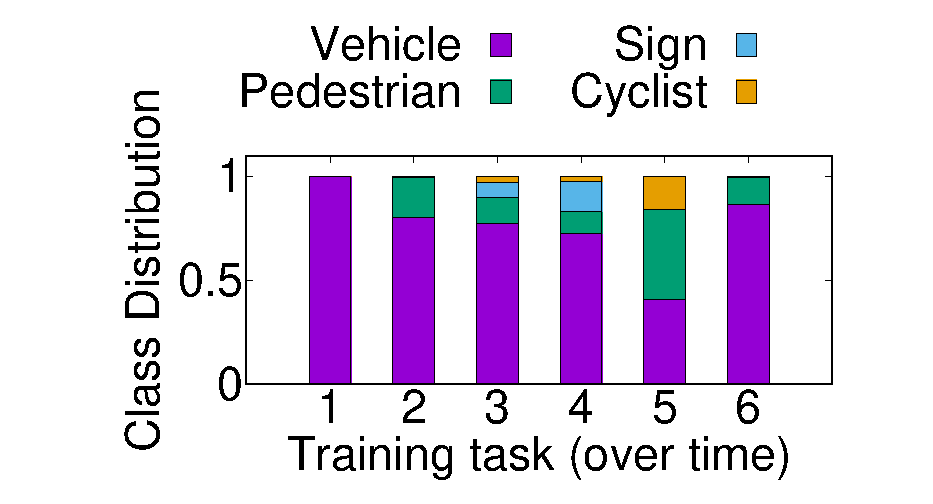
\includegraphics[width=\linewidth]{figures/motivation/Class_Incrementality/new_class.eps}
    \caption{New classes show up over time}
  \end{subfigure}
  ~~
  \begin{subfigure}[t]{0.5\linewidth}
    \centering
    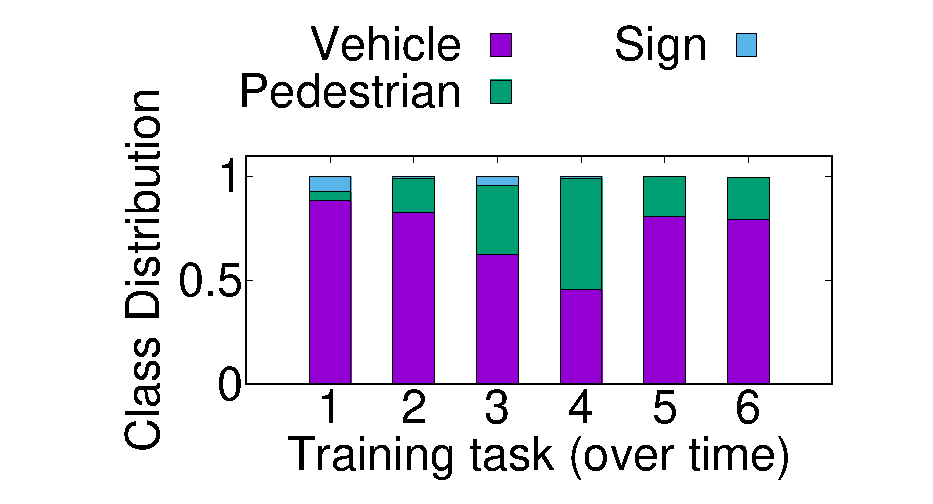
\includegraphics[width=\linewidth]{figures/motivation/Class_Incrementality/class_dist_change.eps} 
    \caption{Class distribution varies over time}
    \label{fig:class-distrib-motivation}
  \end{subfigure}
%   \hfill
  
%   \begin{subfigure}[b]{0.23\textwidth}
%     \centering
%     % 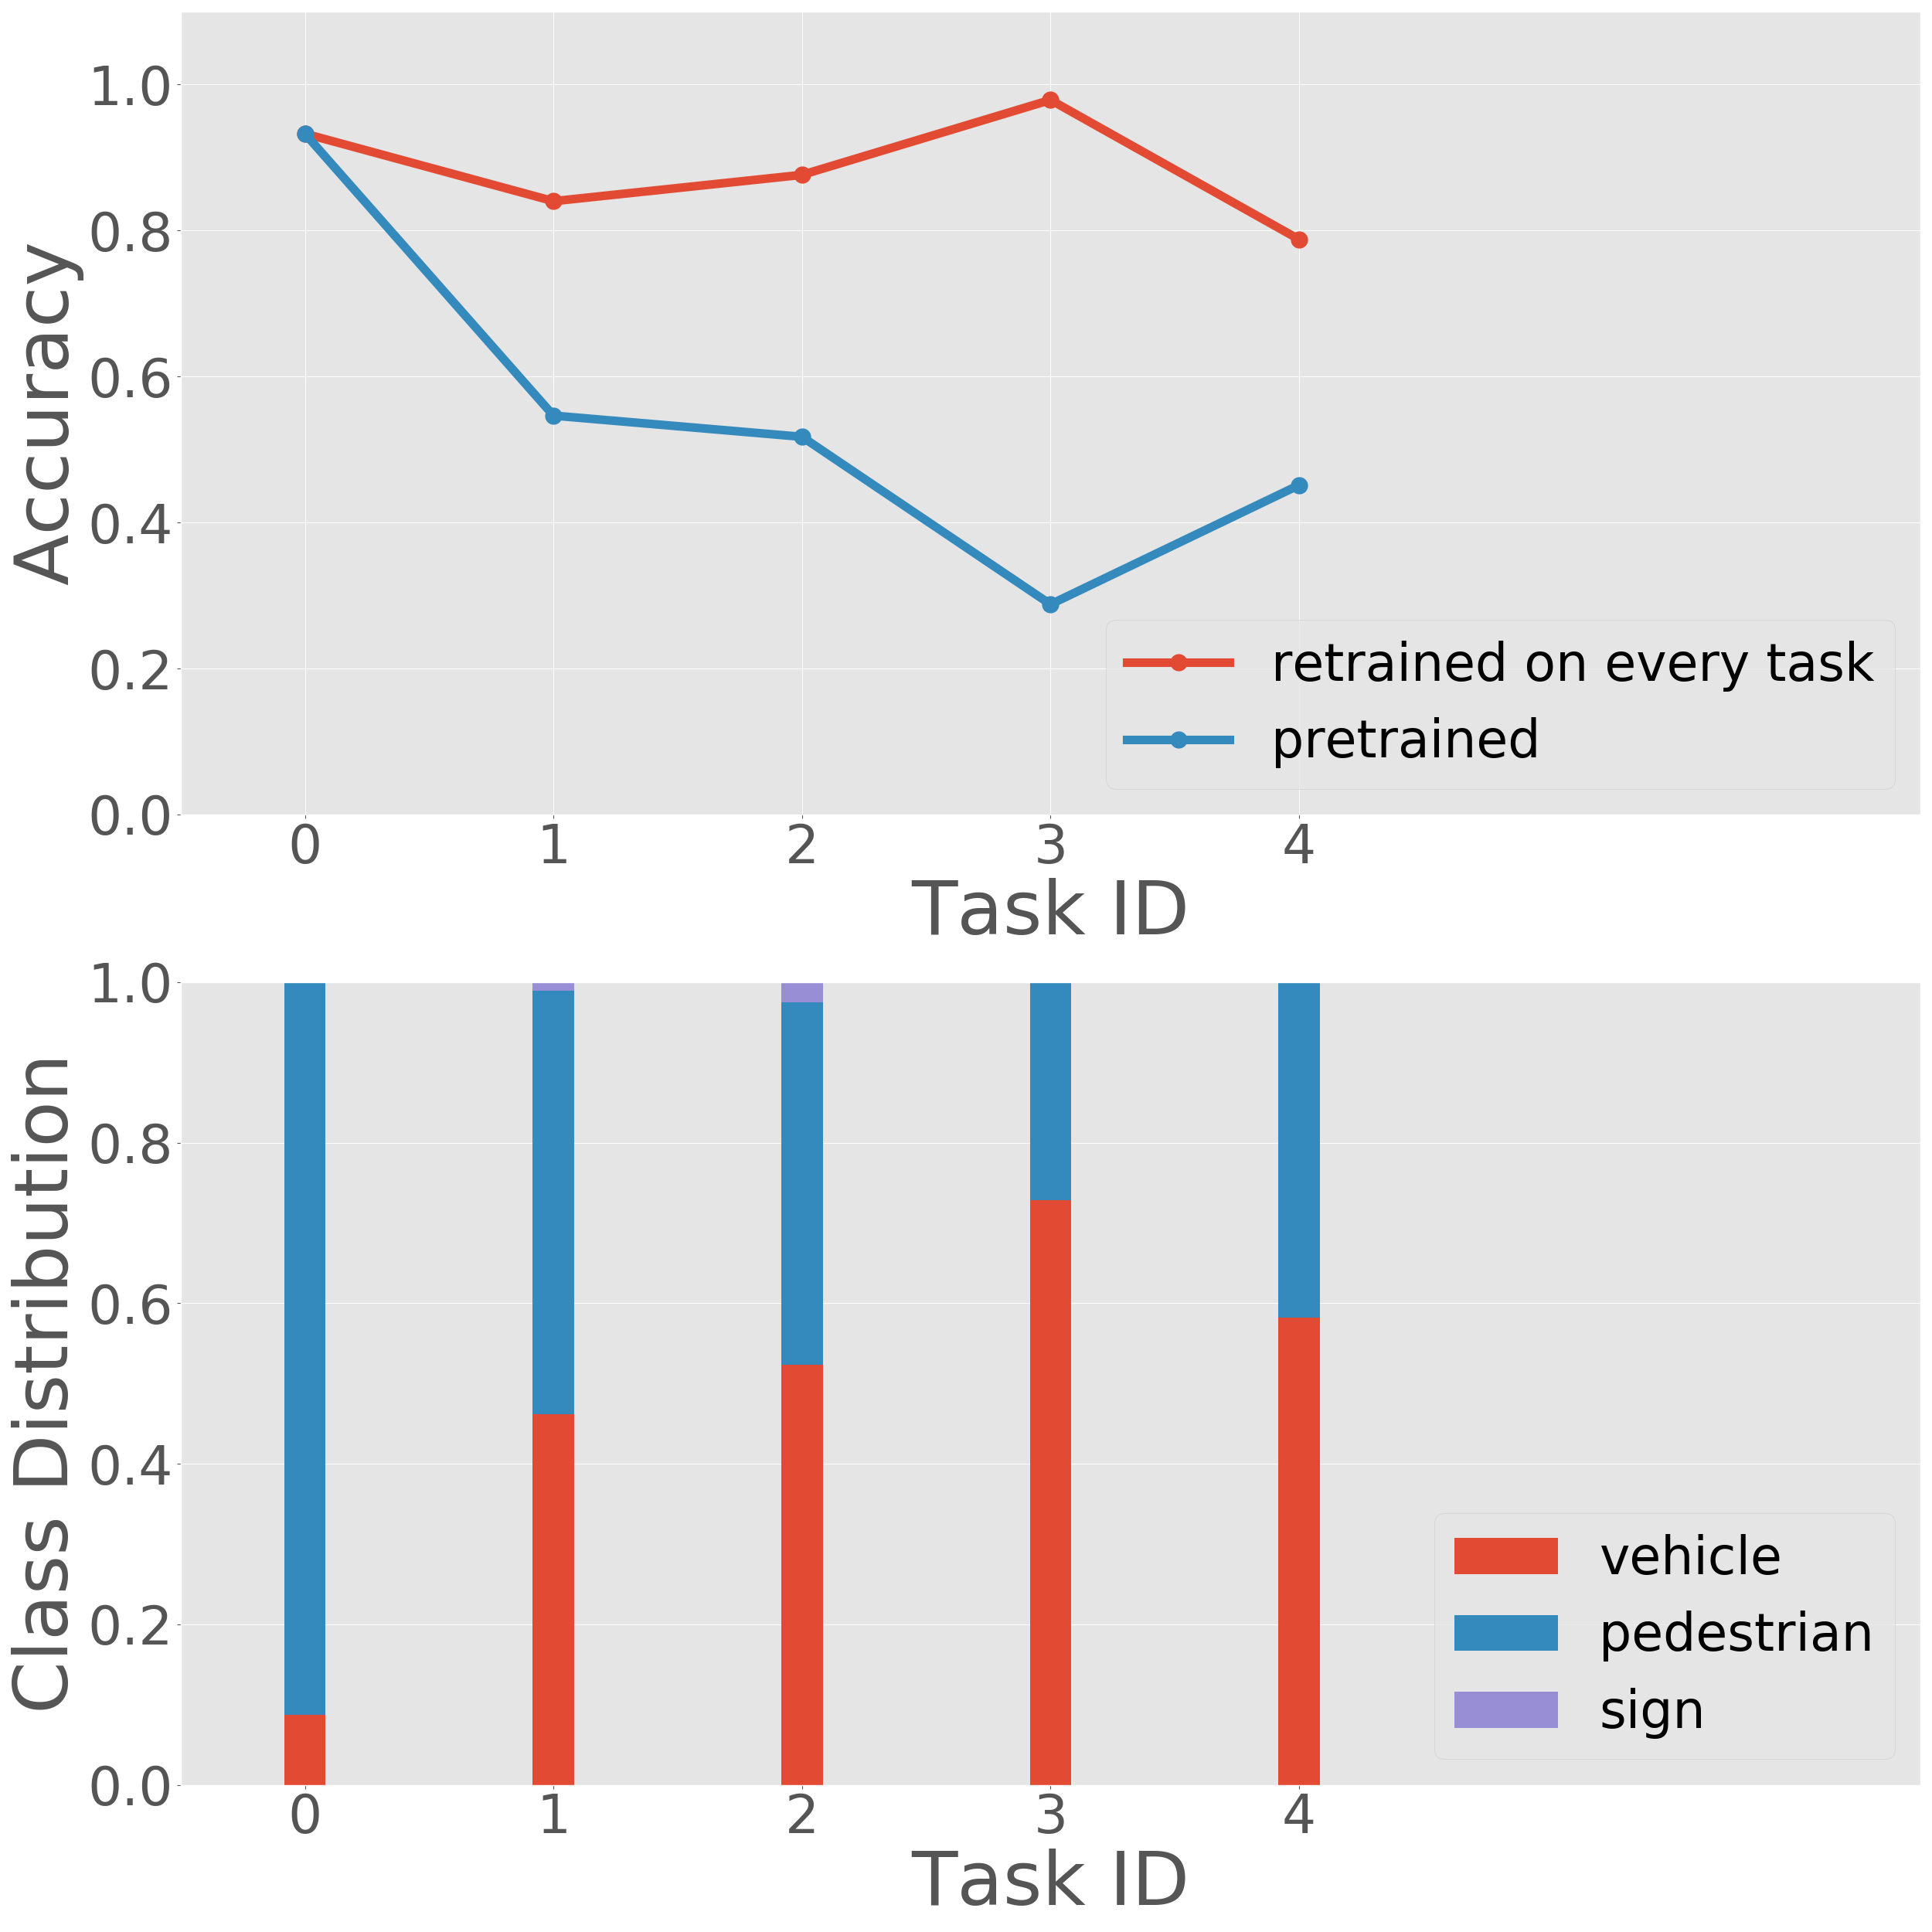
\includegraphics[width=\linewidth]{figures/motivation/Class_Incrementality/class_distribution_change_sf_27.png}
%     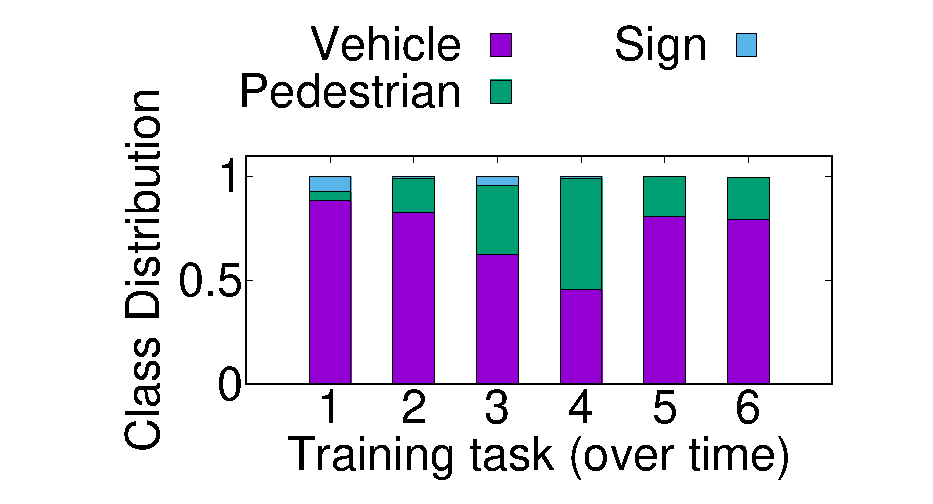
\includegraphics[width=\linewidth]{figures/motivation/Class_Incrementality/class_dist_change.eps}
%     % \caption{Class distribution varies over time}
%     \label{fig:class-distrib-motivation}
%   \end{subfigure}
  \caption{Class incremental learning with Waymo.  \ga{(a) Can we increase to more tasks? are there cyclists at all?} \ga{(b) are there only two classes in this figure, can we have an example of class distrib changing with more classes?}}
  \label{fig:waymo-motivation}
\end{figure}


{\em Class-incremental} training refers to learning about new object classes with time, thus expanding the model's classification targets. Figure \ref{fig:waymo-motivation} motivates class-incrementality where data samples of {\em new classes} are available to the training over time. For instance, the initial training data only consists of samples of vehicles, but over time, pedestrians, road signs, and cyclists are added (Figure \ref{fig:new-classes-motivation}, bottom). Continuously updating the ResNet18 model to include these classes consistently results in higher accuracy (Figure \ref{fig:new-classes-motivation}, top). 

Further, continuous learning is also beneficial when the {\em distribution} of classes changes over time; Figure \ref{fig:class-distrib-motivation}. While the initial training samples are dominated by pedestrians, more examples of vehicles become available with time (Figure \ref{fig:class-distrib-motivation}, bottom). The continuously trained model better copes with this change to achieve higher accuracy (Figure \ref{fig:class-distrib-motivation}, top). 




\begin{figure}[t]
  \centering
  \begin{subfigure}[t]{0.5\linewidth}
    \centering
    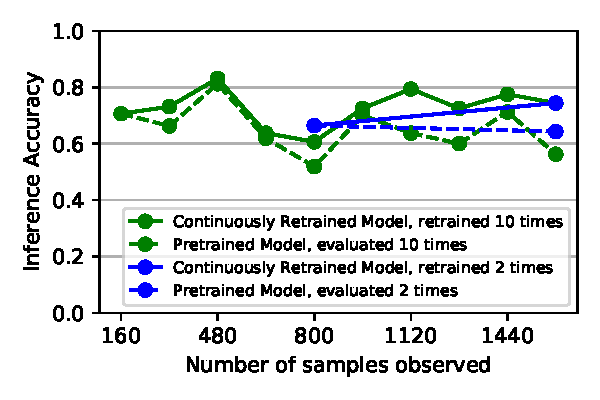
\includegraphics[width=\linewidth]{figures/motivation/incr_learn_tasksize/motivation_tasksize_cologne.pdf}
    \caption{Cologne}
    \label{fig:cologne-motivation}
  \end{subfigure}  
  ~~
  \begin{subfigure}[t]{0.5\linewidth}
    \centering
    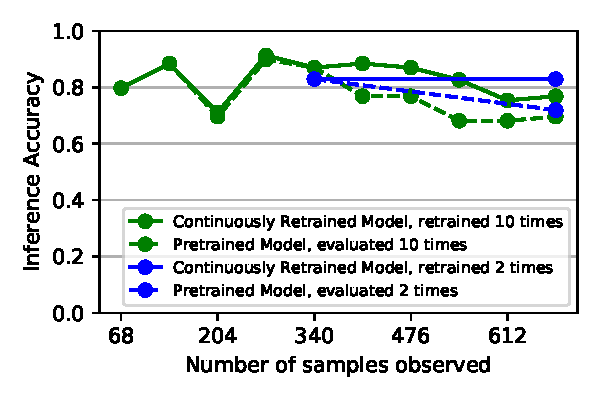
\includegraphics[width=\linewidth]{figures/motivation/incr_learn_tasksize/motivation_tasksize_erfurt.pdf}
    \caption{Erfurt}
    \label{fig:erfurt-motivation}
  \end{subfigure}
  \caption{Cases when a high retraining frequency is detrimental. In the first half of \ref{fig:erfurt-motivation} uptil 340 samples, retraining does not improve the model and must be thus deprioritized in favor of less frequent retraining. \romil{Show larger gap in accuracy - new expt.}}
  \label{fig:cityscapes-frequency-motivation}
\end{figure}

% impact of different retraining frequencies - show variation across two cities
\textbf{Retraining Frequency.} As a model specializes for a specific data distribution, its performance on general data decreases.  Moreover, frequent retraining requires more resources, which may not be available and thus the model may be trained only for a shorter duration \romil{The inference-resource-opportunity-cost argument can also be put here, but is not reflected in the plots}. Thus, a high retraining frequency can reduce the model accuracy.
% \junchen{i like the point that retraining too frequently would backfire, but we probably should explain what determines the benefit of retraining frequently in the first place. again, this is a cost-benefit analysis. this paragraph highlights the cost (of retraining frequently); the benefits (to cope with scene changes?) need to be highlighted as well.}
\junchen{Is retraining too frequently lowers the accuracy because of more frames being dropped or because of retraining ending prematurely for lack of resource? if so, please make it explicit. i was confused as reader..}
This is observed in \cref{fig:cologne-motivation} and \cref{fig:erfurt-motivation}, where having just 2 tasks \romil{Explain what a task is} has a mean accuracy of 70.4\% over the entire dataset, but decreases to 69.8\% when retrained over 10 tasks. Similar behavior for Erfurt (82.9\% vs 82.2\%). \ga{Update the results as per our discussion on email.}
% romilb: Add reference to fig 1 to see cases where high frequency improves the model
% romilb: Show that the same frequency can have different results on different cities. Bar chart?

% golden model; can retain more info but is expensive; edge model's capacity is less but is cheaper to execute
% show graph - golden, edge w/ retraining, edge w/o retraining (for one of the above cities); both sample and class incremental
% romilb: a third line in figure 1 - (showing continuously high accuracy?) 

\noindent{\bf Golden model.}


\subsection{Edge Compute Servers}
\label{subsec:edge}

% edge computing setup: managed edge outposts & their specs, processing videos in a building or campus; typical video streams/edge
Edge computing is central to video analytics deployments \cite{ieee-computer, edge1, edge2} in production. The edge compute is either on private servers that are managed by the enterprises themselves, or is rented from cloud providers whose business contract involves maintaining the edge servers \cite{aws-outpost, azure-stack-edge}. Computation on the edge servers is typically using containers that are orchestrated by frameworks like Kubernetes \cite{kubernetes}. Our study of many enterprise edge deployments indicate that the above mentioned setup of edge {\em servers} are more popular than {\em on-camera} edge devices (cameras with compute on-board) %due to ease of maintenance and amortization of cost when analyzing multiple video streams 
\cite{something}. %Video analytics applications are usually composed of a pipeline of one or more containers that work together \cite{rocket-github}. 
A typical edge server supports analytics on tens of video streams, e.g., from cameras in an enterprise building, that execute in parallel using video analytics pipelines \cite{rocket}. 

% bandwidth and privacy reasons; point to prior work
Video analytics applications adopt edge computing for the reasons of limited network bandwidth to the cloud, unreliability of the network connection to the cloud, and privacy of video content being analyzed. Edge deployments are often in locations that cannot support continuous upload of (high-definition) video streams to the cloud for processing, e.g., in oil rigs with expensive satellite connectivity or automated cars with data-limited cellular connectivity. Further, the network uplinks out of these locations often have outages and thus edge computation provides robustness against these network outages \cite{chick-fill}. Finally, videos often contain sensitive data that users do not want to send to the cloud (e.g., in many EU cities, traffic videos are mandated to be processed on the edge and not sent to the cloud \cite{sweden}). Overall, {\em edge deployments for video analytics is cost-effective, robust, and private}, as has been observed by several prior works \cite{edge, compute, references}. 

% used for inference already; we propose running training too; storage isn't a concern but compute is limited; the network is also a worry, so we cannot access the infinite compute in the cloud
Our proposal is to extend the edge servers, which already performs video DNN inferences, to {\em include continuous training of the edge DNN models}. As \S\ref{subsec:continuous} showed, continuous training of models copes with the data drift and leads to higher inference accuracy. Edge servers already have capacity to store the limited amount of video data that is required for continuous retraining. However, its compute capacity is a concern as the edge server's compute is already provisioned for the DNN inference on live video streams. Since retraining is periodic, i.e., its compute requirements are bursty in nature, provisioning compute resources for retraining will lead to wasted utilization and cost (by as much as \gaa{XXX} in our experiments). For the reasons explained above regarding bandwidth constraints and privacy sensitivities, transmitting the videos to the cloud for retraining is not preferred.

% objective of inference and retraining on edge for multiple video streams
Our objective is to support both live video analytics inference of DNN models as well as continuous training of these models. As we describe next, we develop techniques to minimize disruption to the inference workloads while smartly allocating resources for continuous retraining. %maximize the eventual inference accuracy. 

\junchen{i like the flow of 2.2 but overall 2.2 seems repetitive to the edge-related arguments at the beginning of 2.1.}

\junchen{here's a slightly different way to organize it: 
\begin{itemize}
    \item 2.1 Towards accurate DNN inference at the edge
    \begin{itemize}
        \item deploying cheap DNN at edge is increasingly common and necessary. (merge 1st para and 1st half of 2.2)
        \item cheap model re-trained with in-situ data can often strike a better compute-accuracy tradeoff (assuming data distribution doesn't change!) (we don't have a graph to support it for now, but i feel its necessary and isn't hard to get one).
    \end{itemize}
    \item 2.2 Need for continuous retraining
    \begin{itemize}
        \item data drift is common and could be handled with continuous retraining. (the paragraphs under ``data drifts'')
        \item retraining is too frequently can backfire. (the ``retraining frequency'' part)
    \end{itemize}
This section should end with the need for resource-efficient continuous retraining at edge, which the next section will elaborate in more details.
\end{itemize}}